% \relatorio

% {Análise da acessibilidade após possível intervenção na Rua Uberabinha
% }
% {
%     \noindent Pesquisadores: Isabella Daccache, João Vitor Heinke, João Vitor Rocha e Lucca Kao
    
%     \noindent Orientador: Laura Janka, Natascha Vital e Heloisa Escudeiro
% }
% {
%    Com o objetivo de transformar os espaços públicos mais verdes e próprios para pedestres e ciclistas, o projeto "Repensando Espaços Públicos – Rua Uberabinha" estuda transformar uma rua local em uma praça pública. Dessa forma, o presente estudo busca investigar as consequências para a acessiblidade das modalidades de transporte (carro, bicicleta e pedestres) após uma possível implementação do projeto localizado no bairro Itaim em São Paulo. A partir desta pesquisa é possível concluir que desconsiderando o trânsito, a área de alcance dos tipos de transporte não seriam afetadas, além de que 30,78\% das rotas de pedestres e 61,19\% de ciclistas seriam beneficiados ou não sofreriam alterações, enquanto 69,10\% das rotas de carro seriam prejudicadas ou não sofreriam alterações.
% }
% {
% Uberabinha, acessibilidade, isócrona, oportunidade
% }

\relatorio
{Análise da acessibilidade após possível intervenção na Rua Uberabinha}
{

    \noindent \textbf{Políticas Públicas}
    
    \noindent Pesquisadores: Isabella Daccache, João Vitor Heinke, João Vitor Rocha e Lucca Kao
    
    \noindent Orientadoras: Laura Janka, Natascha Vital e Heloisa Escudeiro

}
{

   Com o objetivo de transformar os espaços públicos mais verdes e próprios para pedestres e ciclistas, o projeto "Repensando Espaços Públicos – Rua Uberabinha" estuda transformar uma rua local em uma praça pública. Dessa forma, o presente estudo busca investigar as consequências para a acessiblidade das modalidades de transporte (carro, bicicleta e pedestres) após uma possível implementação do projeto localizado no bairro Itaim em São Paulo. A partir desta pesquisa é possível concluir que desconsiderando o trânsito, a área de alcance dos tipos de transporte não seriam afetadas, além de que 30,78\% das rotas de pedestres e 61,19\% de ciclistas seriam beneficiados ou não sofreriam alterações, enquanto 69,10\% das rotas de carro seriam prejudicadas ou não sofreriam alterações.
}
{
Uberabinha, acessibilidade, isócrona, oportunidade
}


\section{Introdução}

A palavra ``acessibilidade'' em meio a discussão do dia a dia provavelmente acarretará em um ponto de vista sobre acessibilidade de pessoas detentoras de alguma deficiência motora ou cerebral, e de modo visual, a lembrança do quadrado azul com o desenho de um cadeirante. No entanto, a palavra possui cunho mais genérico do que usualmente é utilizada, com outro significado para a palavra, \textcite{vieira2006} apresenta o seguinte conceito: “A acessibilidade é o acesso fácil, qualidade do que é acessível. A falta de acessibilidade no transporte coletivo está associada as grandes distâncias e longas viagens”. Dessa forma, o presente estudo concentrará esforços para compreender a acessibilidade viária nos arredores do bairro Itaim Bibi, São Paulo, mais especificamente com ponto central o Insper – Instituto de Pesquisa e Ensino localizado na rua Quatá.

Em 2014, a cidade de São Paulo recebeu um novo direcionamento na sua organização viária e urbana, em outras palavras, atualizou seu Plano Diretor, o qual não era alterado desde 2002. Neste ano, portanto, São Paulo propôs ideias primárias sobre a construção de uma cidade mais inclusiva e acessível para modos de transporte que ultrapassassem o veículo particular, ou seja, a busca por uma maior acessibilidade para pedestres e ciclistas. Propostas essas que enfatizavam a construção de mais áreas verdes, transformação de logradouros em praças públicas, aumentando assim, os espaços de convivência e a segurança viária do público alvo. 

Esses aspectos enfatizados no Plano Diretor de 2014, foram matrizes da construção do projeto “Repensando Espaços Públicos – Rua Uberabinha” da Gestão Urbana da cidade de São Paulo. Projeto este que reuniu diversas ideias de transformação no logradouro, buscando acrescentar características as quais são citadas no Plano Diretor. Algumas das ideias apresentadas foram: criação de um espaço público de encontro e convívio; intervenções que garantam segurança na caminhabilidade do local e oferta de comércio e serviços, ações essas que bloqueariam a rua para a passagens de carros, focalizando tal espaço para pedestres e ciclistas.

De tal modo, tendo em vista o fluxo diário na rua local do bairro do Itaim por conta de instituições de ensino nos arredores do logradouro, como, Instituto de Ensino e Pesquisa e Universidade Anhembi Morumbi, este estudo compreende a relevância do impacto de tal decisão e busca esclarecer as consequências para cada uma das modalidades de transporte, tendo como localidade principal de análise o Insper.


\section{Revisão Literária}

Em busca de exemplos similares a tal decisão, a literatura apresenta duas importantes questões: dificuldade sobre a mensuração do conceito de acessibilidade; compreensão sobre o modo de interação e envolvimento entre o espaço analisado e seus usuários. Isto é, a literatura sobre estruturas viárias possui poucas metodologias elaboradas e aprovadas pela academia sobre a mensuração e comparação entre a acessibilidade de um local e outro, ou uma possível estrutura viária e sua alternativa. Ademais, sob o ponto de vista do urbanismo, decisões como da Rua Uberabinha ultrapassam barreiras de análises absolutas, permeando um âmbito mais humano e que envolve um certo conhecimento empírico.

Primeiramente com relação ao entendimento do vínculo entre o espaço e os usuários, o urbanismo atesta que de modo descritivo é necessária a concepção sobre o uso do espaço no momento presente. Em outras palavras, a construção e planejamento de lugares deve ser sob a perspectiva da colaboração, a partir da expertise da comunidade local, que busca seu próprio bem-estar, ponto de vista este dominado a partir da metodologia do \textit{Place Making} \textcite{Melo2024}.

Tendo em vista que tal método se baseia por completo em competências humanas, para a contagem e compreensão sobre o uso do espaço pelos indivíduos, a validade dos resultados gerados é duvidosa. Isto pois, o foco e assertividade de uma pessoa na contagem de carros, pedestres, ciclistas e motociclistas não é alta, o que cria uma incerteza sobre tal. Dessa forma, é discutível a robustez de estudos baseados no Place Making, com uma possibilidade de melhora de tais a partir do uso de diferentes técnicas de contagem. \textcite{jantsch2020} apresenta de modo conciso e claro essa dificuldade da contagem manual em comparação ao uso de tecnologias, analisando o erro de cada método e seus benefícios e malefícios. Não só ele, como \textcite{osinski2020} demonstram outro método mais complexo de contagem, porém mais prático, a partir do uso de algoritmos de visualização de imagens de trânsito.

Por outro lado, com um ponto de vista microeconômico \textcite{koenig1980}, apresenta um método de mensuração da acessibilidade de um local a partir de duas maneiras diferentes: isócronas e somatório de oportunidades. O primeiro, isócronas, define de forma cartográfica a área de alcance de uma pessoa, partindo de um ponto de origem utilizando uma modalidade de transporte específica, apresentando uma comparação da área de alcance entre as modalidades. Ou seja, um método que metrifica a acessibilidade como sinônimo do alcance obtido a depender da origem e o transporte utilizado, um exemplo disso é retratado na Figura \ref{fig:isocrona}. No exemplo fictício citado, a origem é representada pelo ponto preto, que é rodeado por duas áreas, azul clara e escura, as quais representam o alcance que uma pessoa teria em 10 e 20 minutos de deslocamento, respectivamente, utilizando uma bicicleta.

\begin{figure}[H]
    \centering
    \caption{Exemplo isócrona}
    \includegraphics[width = 0.6\linewidth]{relatorios/uberabinha/figuras/exemplo_isocrona.png}
    \label{fig:isocrona}
\end{figure}

Uma definição pragmática para o conceito de isócrona é apresentado pelo \textcite{esri_isochrone}: ``Uma linha em um mapa conectando pontos de tempo percorrido igual, especialmente, tempo de viagem para ou de uma localização fornecida.''

Outro método de análise sobre a acessibilidade levantado por Koenig é a partir da somatória das oportunidades entre uma origem \textit{i} e seus possíveis destinos \textit{j}. Essa metodologia é melhor representada pela expressão matemática \ref{expressao_micro}:

\begin{equation}
\label{expressao_micro}
    A_i = \sum_j O_j f(C_{ij})
\end{equation}

Com relação aos elementos da expressão o primeiro $O_j$ se refere ao número de oportunidades existentes no destino \textit{j}. Já a função $f(C_{ij})$, traduz a função de impedância, elemente este que pondera as oportunidades de acordo com a rota \textit{ij}, utilizada. Desse modo, o somatório de todas as oportunidades ponderadas mensuram a acessibilidade do local \textit{i}, representado por $A_i$.

O raciocínio contido em tal expressão é compreendido da seguinte maneira. O ponto de origem \textit{i} é o local de estudo de interesse, o qual está sendo analisado sua acessibilidade. Após o recorte da área de estudo desejada, seja essa um raio de 3Km ao redor do local de origem, ou uma região de logradouros nos arredores da origem, é necessário o levantamento de todas as oportunidades presentes nessa área. O conceito de oportunidade não é especificado por Koenig em seu estudo, e portanto, para a atual pesquisa este será utilizado em referência a localidades onde uma pessoa poderia interagir e obter um bem-estar/felicidade. Em outras palavras, supermercados, restaurantes, academias, shoppings foram alguns dos estabelecimentos reconhecidos pelos estudos como oportunidades a serem localizadas na área de estudo.

Dessa forma, a análise se aplica sobre cada caminho realizado entre a origem \textit{i}, o destino \textit{j}, a quantidade de oportunidades que o indivíduo teria de acesso no destino, sendo toda essa expressão ponderada por uma função de impedância do caminho. A ideia central é de que, ao se deslocar de \textit{i} para \textit{j} o indivíduo tenha uma felicidade, e essa felicidade é interferida pelo caminho utilizado, sofrendo prejuízos caso a impedância seja maior. Impedância neste contexto pode ser entendida como resistência, sendo, portanto, um fator inversamente proporcional a acessibilidade de um local, de modo que quanto maior a impedância em tais rotas, menos acessível seria o local. Os fatores contidos na função de impedância são inúmeros, porém para melhor compreensão da metodologia, exemplos desses fatores são, distância percorrida, tempo do trajeto e segurança da rota. Logo, quanto maior a distância percorrida, ou quanto maior o tempo do trajeto, ou até quanto maior a taxa de assaltos e furtos na rota utilizada, maior a impedância do específico trajeto \textit{ij}, e assim, menos acessível é o local.

Tendo isso em vista, a hipótese que os modelos de Koenig propõe para a situação de análise sobre a possível intervenção na Rua Uberabinha podem ser divididas em dois grupos. Para o grupo de indivíduos que fazem uso da região baseando-se em transportes de carro, a hipótese é de que a alteração afetaria negativamente ou não teria nenhum efeito sobre a acessibilidade desse tipo de transporte, isto pois, o fechamento da rua mudaria todas as rotas que passavam por tal rua, o que aumenta a distância de deslocamento, e assim, aumentaria a impedância e provavelmente diminuiria a área das isócronas. Contudo, o presente estudo não buscou quantificar essa impedância, mas é claro a partir da metodologia que esse efeito seria negativo ou de magnitude irrisória, sendo impossível um benefício para os carros. 

Já por outro lado, para o grupo de pedestres e ciclistas o fechamento da rua para carros traria um efeito positivo na acessibilidade, uma vez que sem a passagem de carros o espaço se torna mais seguro para pedestres e ciclistas que não necessitarão se atentar a possíveis acidentes. Dessa forma, essa alteração teria efeito positivo ou irrisório, não sendo possível prejudicar os pedestres e ciclistas.

Assim sendo, a hipótese a ser testada empiricamente é se essa alteração viária afeta de alguma forma as isócronas de cada uma das modalidades de transporte. Para além dessa hipótese, o mapeamento das oportunidades que estão ao redor do ponto de origem (Insper), quais são acessíveis para cada tipo de transporte em determinado tempo, e quais utilizam a Rua Uberabinha em suas rotas são objetivos de estudo também.

\section{Metodologia}
Assim como apresentado pela revisão da literatura, o estudo descritivo sobre o local foi feito com o intuito de entender como a população local utiliza o espaço e qual o fluxo de carros, pedestres e ciclistas durante diferentes períodos do dia. Para isso, foram feitas contagens durante períodos de trinta minutos espaçados durante o dia, documentando a quantidade de carros/pedestres/ciclistas que desciam a Rua Quatá ou faziam a conversão na Rua Uberabinha. Os dias de coletas variaram entre duas semanas e diferentes dias da semana, com coletas em quatro dias no total, duas terças-feiras e uma segunda-feira e uma quarta-feira. O intuito de modo geral era buscar entender qual a magnitude do fluxo total diário no local, como também, qual modalidade de transporte mais utilizava o logradouro possivelmente transformado. Esses resultados serão discutidos posteriormente no trabalho, no entanto é interessante ressaltar as incertezas sobre a robustez no modo em que a análise é empregada. 

A realização das contagens para compreensão do fluxo atual no local, de forma manual, é questionável, uma vez que a contagem por um ser humano é repleta de falhas, desatenção o que pode tornar os dados viesados. Como já citado, os períodos de coleta de dados possuíam duração de 30 minutos e esses eram subdivididos entre outros três conjuntos de contagem, buscando reduzir os riscos de erro de contagem. Contudo, para o olho humano, o foco durante dez minutos, analisando e contabilizando quatro diferentes tipos de modalidade de transporte: carro; pedestre; motocicleta e bicicleta, é duvidoso.

A contagem em si foi feita com auxílio do aplicativo Multi-counter, e dividida entre duas pessoas, cada um analisando um fluxo específico, seja este o de continuação na Rua Quatá (Ponto 4) ou conversão na Rua Uberabinha (Ponto 5). As Figuras \ref{fig:rotas} e \ref{fig:app} apresentam respectivamente o ponto de coleta e a interface do aplicativo utilizado.

\begin{figure}[H]
    \centering
    \caption{Local de contagem do estudo}
    \includegraphics[width = 0.6\linewidth]{relatorios/uberabinha/figuras/rotas_analise.png}
    \label{fig:rotas}
\end{figure}

\begin{figure}[H]
    \centering
    \includegraphics[width = 0.4\linewidth]{logo/hlogo.png}
    \caption{Exemplo das contagens no aplicativo - Multi-counter}
    \label{fig:app}
\end{figure}

Para a elaboração das isócronas e análise de acessibilidade sobre as oportunidades que cada tipo de transporte tem acesso em certo espaço de tempo, a ferramenta do r5r foi utilizada. Uma biblioteca da linguagem de programação R, construída por \textcite{pereira_r5r_2021}. Essa auxiliou na construção das isócronas e cálculos sobre distância e tempo de deslocamento do ponto de origem até cada uma das oportunidades mapeadas. Com relação a alteração da estrutura viária e construção dos mapas, essas ações foram feitas utilizando o software de informação geográfica \citefield{QGIS}{title}, a partir dos dados retirados do \citefield{GeoSampa}{title}.

Com relação ao mapeamento de todas as oportunidades ao redor do Insper, foi utilizada a ferramenta \citefield{google_places}{title}. Esta ferramenta retorna uma lista de lugares correspondentes às especificações dentro de um raio estipulado. Para maximizar a identificação de oportunidades, foi criado um filtro específico para os tipos de lugares, dada a ampla variedade disponível na API. 

Foram selecionados os tipos mais relevantes que englobam: \textit{car\_dealer;
car\_rental; car\_repair; car\_wash; gas\_station; parking; farm; school; university; accounting; bank; restaurant; cafe; bar; coffee\_shop; administrative\_area\_level\_1; administrative\_area\_level\_2; fire\_station; police; dentist; doctor; drugstore; hospital; pharmacy; hotel; barber shop; beauty salon; insurance agency; laundry; lawyer; real estate agency; veterinary\_care; market; pet\_store; shoe\_store; shopping\_mall; sporting\_goods\_store; store; supermarket; wholesaler; fitness\_center e gym}.


A pesquisa tomou como premissa um raio de 3 quilômetros como a área de interesse para análise, tendo como centro as coordenadas do Insper. Durante o mapeamento, algumas dificuldades foram enfrentadas, entre elas o número limitado de requisições permitidas. Para contornar essa limitação, o filtro de tipos de lugares foi crucial, além da criação de múltiplas contas do Google para aumentar o número de requisições. Outro desafio foi a quantidade limitada de oportunidades retornadas pela API para cada tipo de lugar dentro do círculo de 3 quilômetros, sendo apenas 20 lugares por tipo. A solução encontrada foi realizar requisições com círculos de raio menor, preenchendo o todo de 3km de raio. 

Dessa maneira, foram utilizados círculos com raios de 200m para mapear toda a área, tendo em alguns espaços a sobreposição de requisições para justamente não existirem áreas não mapeadas. Para evitar duplicidade na lista de oportunidades, foram removidas as entradas repetidas, garantindo que cada oportunidade aparecesse apenas uma vez.
Após possuir todas as oportunidades em um raio de 3Km ao redor do Insper, utilizou-se de outra API \citefield{google_directions}{title}, que nela é possível retornar o caminho que o Google Maps utilizaria de sugestão para sair de um local \textit{X} para um destino \textit{Y}. Realizou-se através de um código Python as requisições necessárias para as 3 diferentes modalidades de transporte presentes na pesquisa: carros, pedestres e bicicletas.

Foi também mapeado, em uma região menos abrangente, a qualidade dos restaurantes da região, buscando compreender a necessidade dos indivíduos de se deslocar mais de 1Km no horário do almoço. Tal detalhamento foi elaborado com auxílio da \citefield{google_geocoding}{title} para obter o \textit{place id} de cada local, com base em sua latitude e longitude. Com essa informação, foi possível obter a avaliação de cada restaurante, permitindo assim uma análise de como os melhores restaurantes se distribuem na região.

\section{Resultados}
Os dados coletados durante as contagens ao final do estudo não foram considerados, isto pois como foi discutido na seção de metodologia, a validade das coletas era questionável. Por conta de uma escolha errônea na distribuição das coletas, a interpolação dos dados, para melhor visualização do fluxo diário foi impossibilitada, tornando a base de dados não robusta.

Por outro lado, a construção das isócronas trouxe resultados interessantes. Nas Figuras \ref{fig:iso_car_C}, \ref{fig:iso_bike_C} e \ref{fig:iso_pe_C}, é possível analisar as isócronas de cada modalidade de transporte. De modo descritivo, os resultados são próximos do óbvio, a área de alcance do carro e da bicicleta são muito maiores que a área de alcance do pedestre, simplesmente por conta da velocidade de deslocamento que estes conseguem alcançar. Um ponto necessário a ser enfatizado sobre tais resultados é de que essas isócronas não estão considerando o trânsito como um elemento de análise.

\begin{figure}[H]
    \centering
    \caption{Isócrona Carro sem intervenção na Rua Uberabinha}
    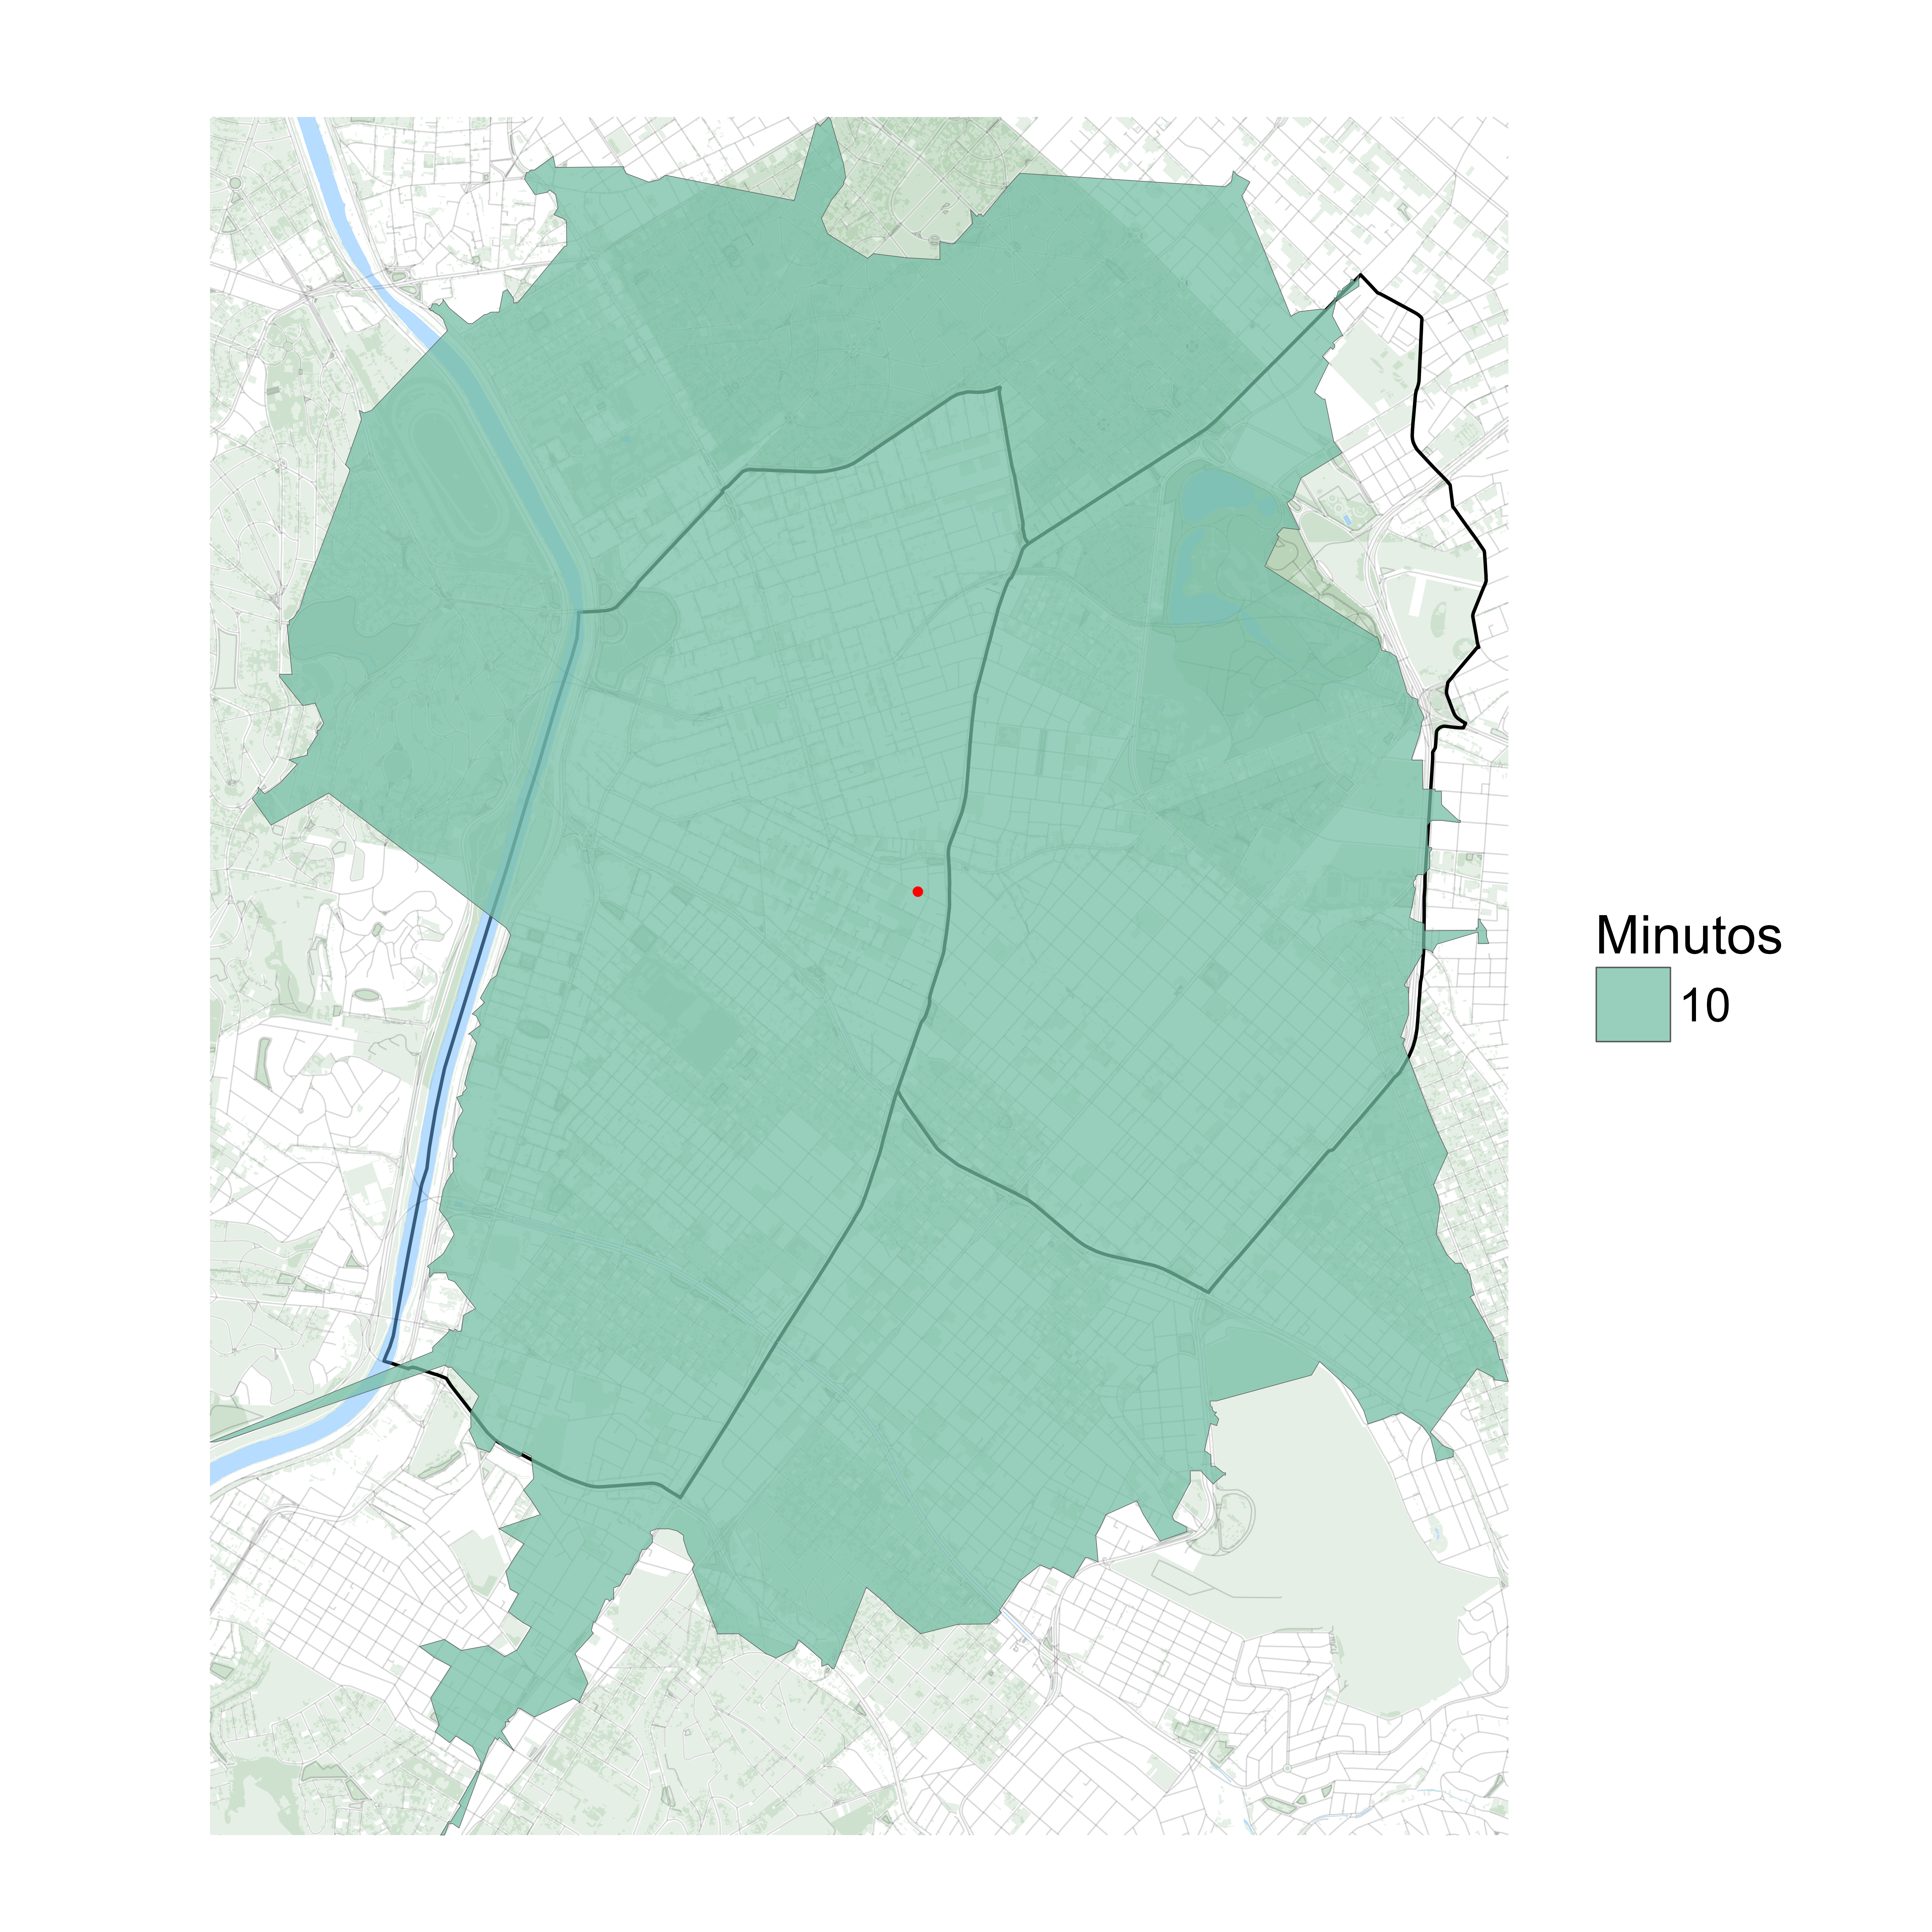
\includegraphics[width = 0.8\linewidth]{relatorios/uberabinha/figuras/car_C_uber_FINAL.png}
    \label{fig:iso_car_C}
\end{figure}

\begin{figure}[H]
    \centering
    \caption{Isócrona Bicicleta sem intervenção na Rua Uberabinha}
    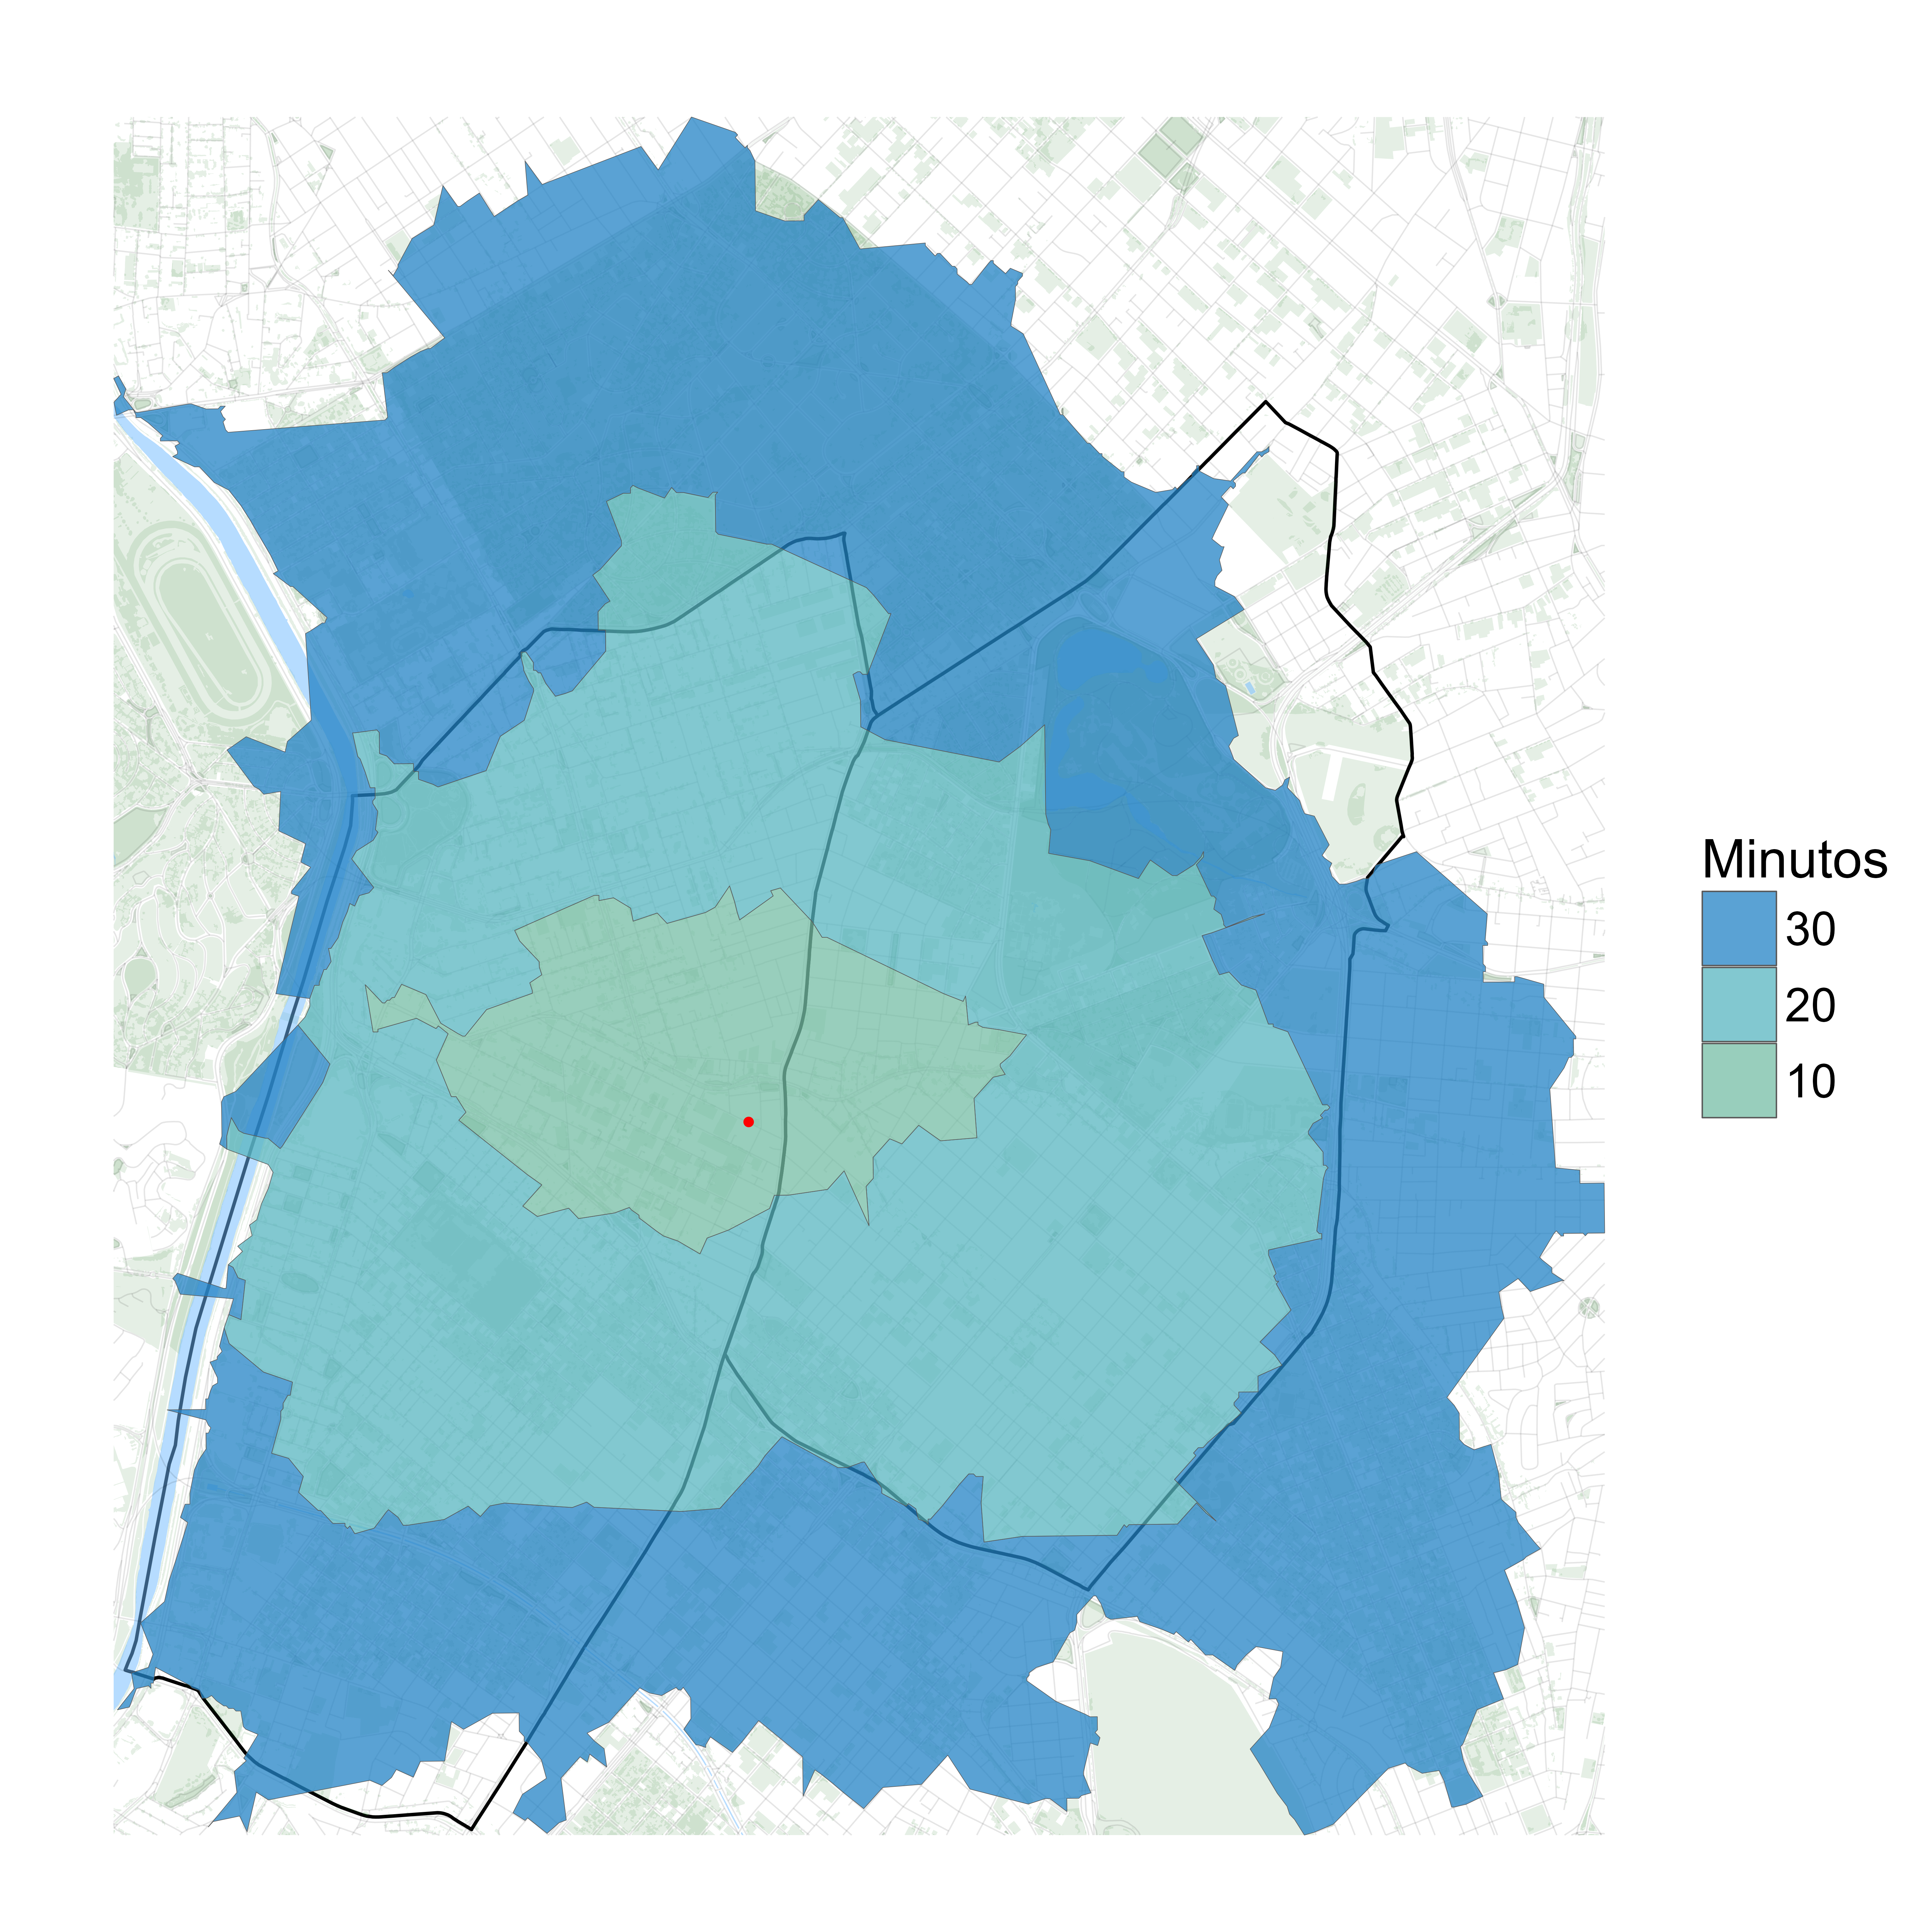
\includegraphics[width = 0.8\linewidth]{relatorios/uberabinha/figuras/bike_C_uber_FINAL.png}
    \label{fig:iso_bike_C}
\end{figure}

\begin{figure}[H]
    \centering
    \caption{Isócrona Pedestre sem intervenção na Rua Uberabinha}
    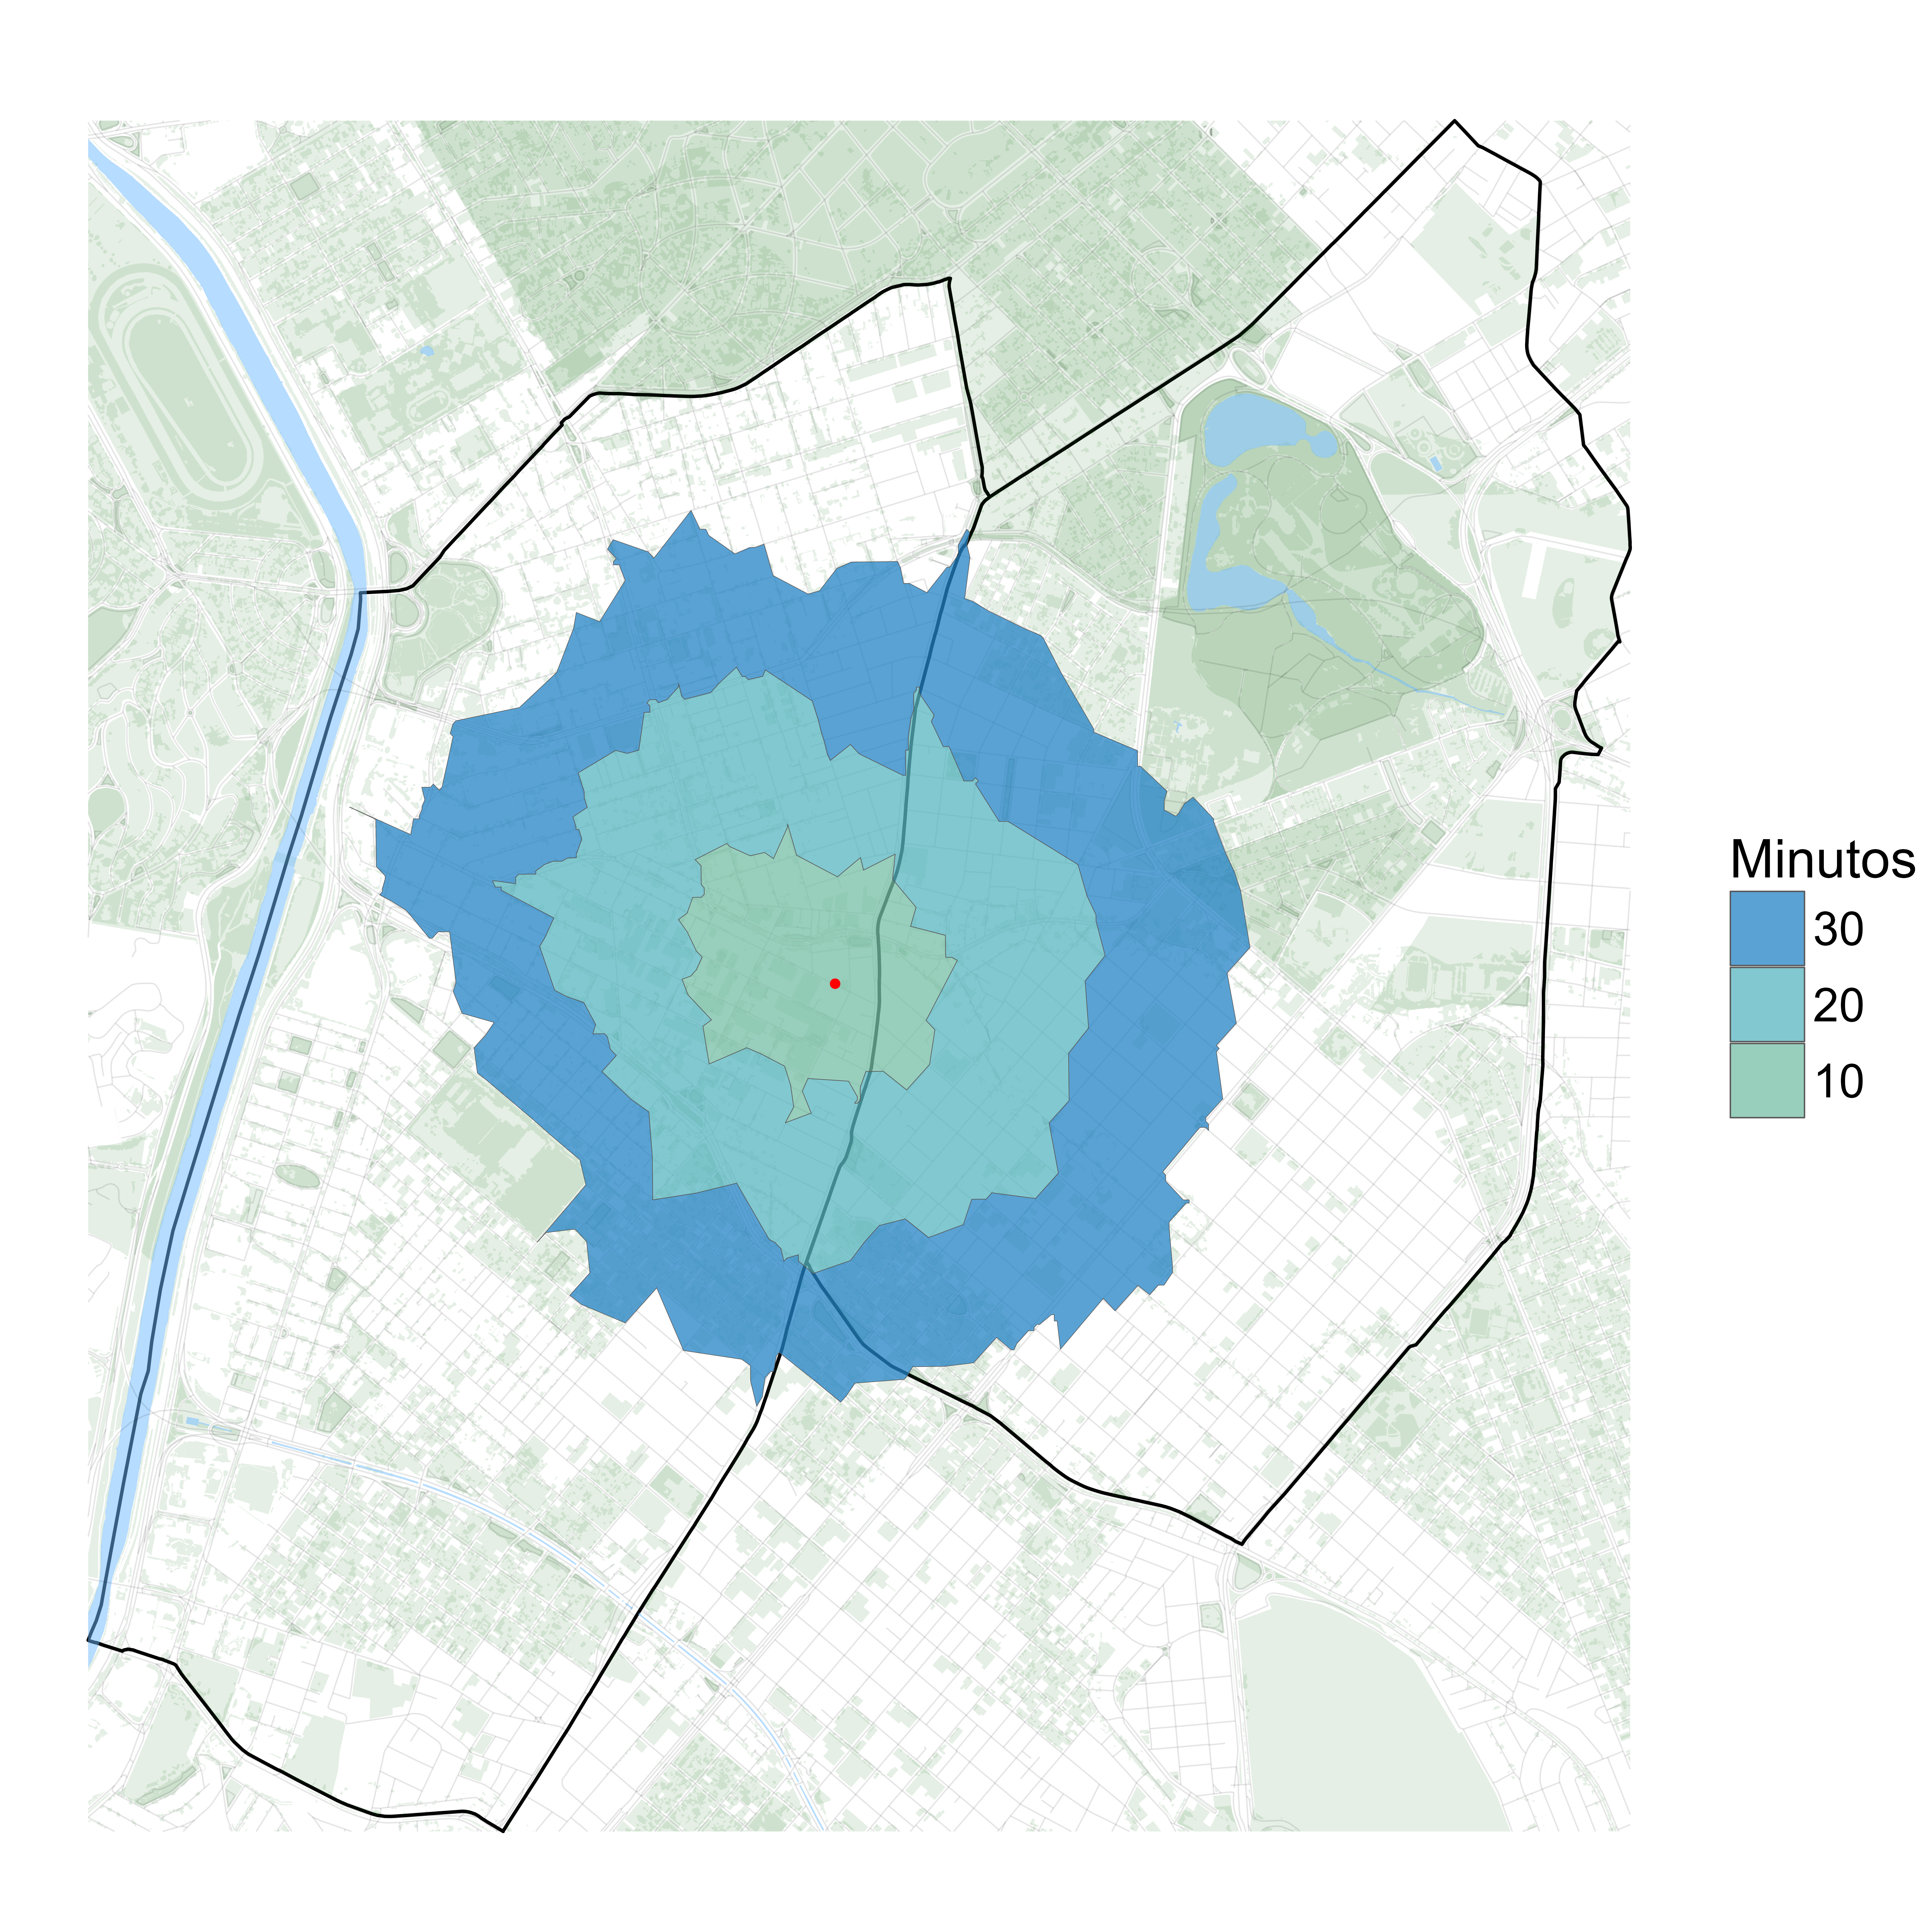
\includegraphics[width = 0.8\linewidth]{relatorios/uberabinha/figuras/walk_C_uber_FINAL.png}
    \label{fig:iso_pe_C}
\end{figure}

Já nas Figuras \ref{fig:iso_car_S}, \ref{fig:iso_bike_S}, \ref{fig:iso_pe_S} estão apresentadas as isócronas de cada modalidade de transporte com a possível alteração na Rua Uberabinha, isto é, impossibilidade de carros circularem em tal espaço. Com base na comparação entre as isócronas, é possível compreender que a diferença sobre o alcance dos tipos de transporte quando é feita a alteração na estrutura viária é irrisória, não representando nenhum benefício ou malefício de magnitude considerável.

\begin{figure}[H]
    \centering
    \caption{Isócrona Carro com intervenção na Rua Uberabinha}
    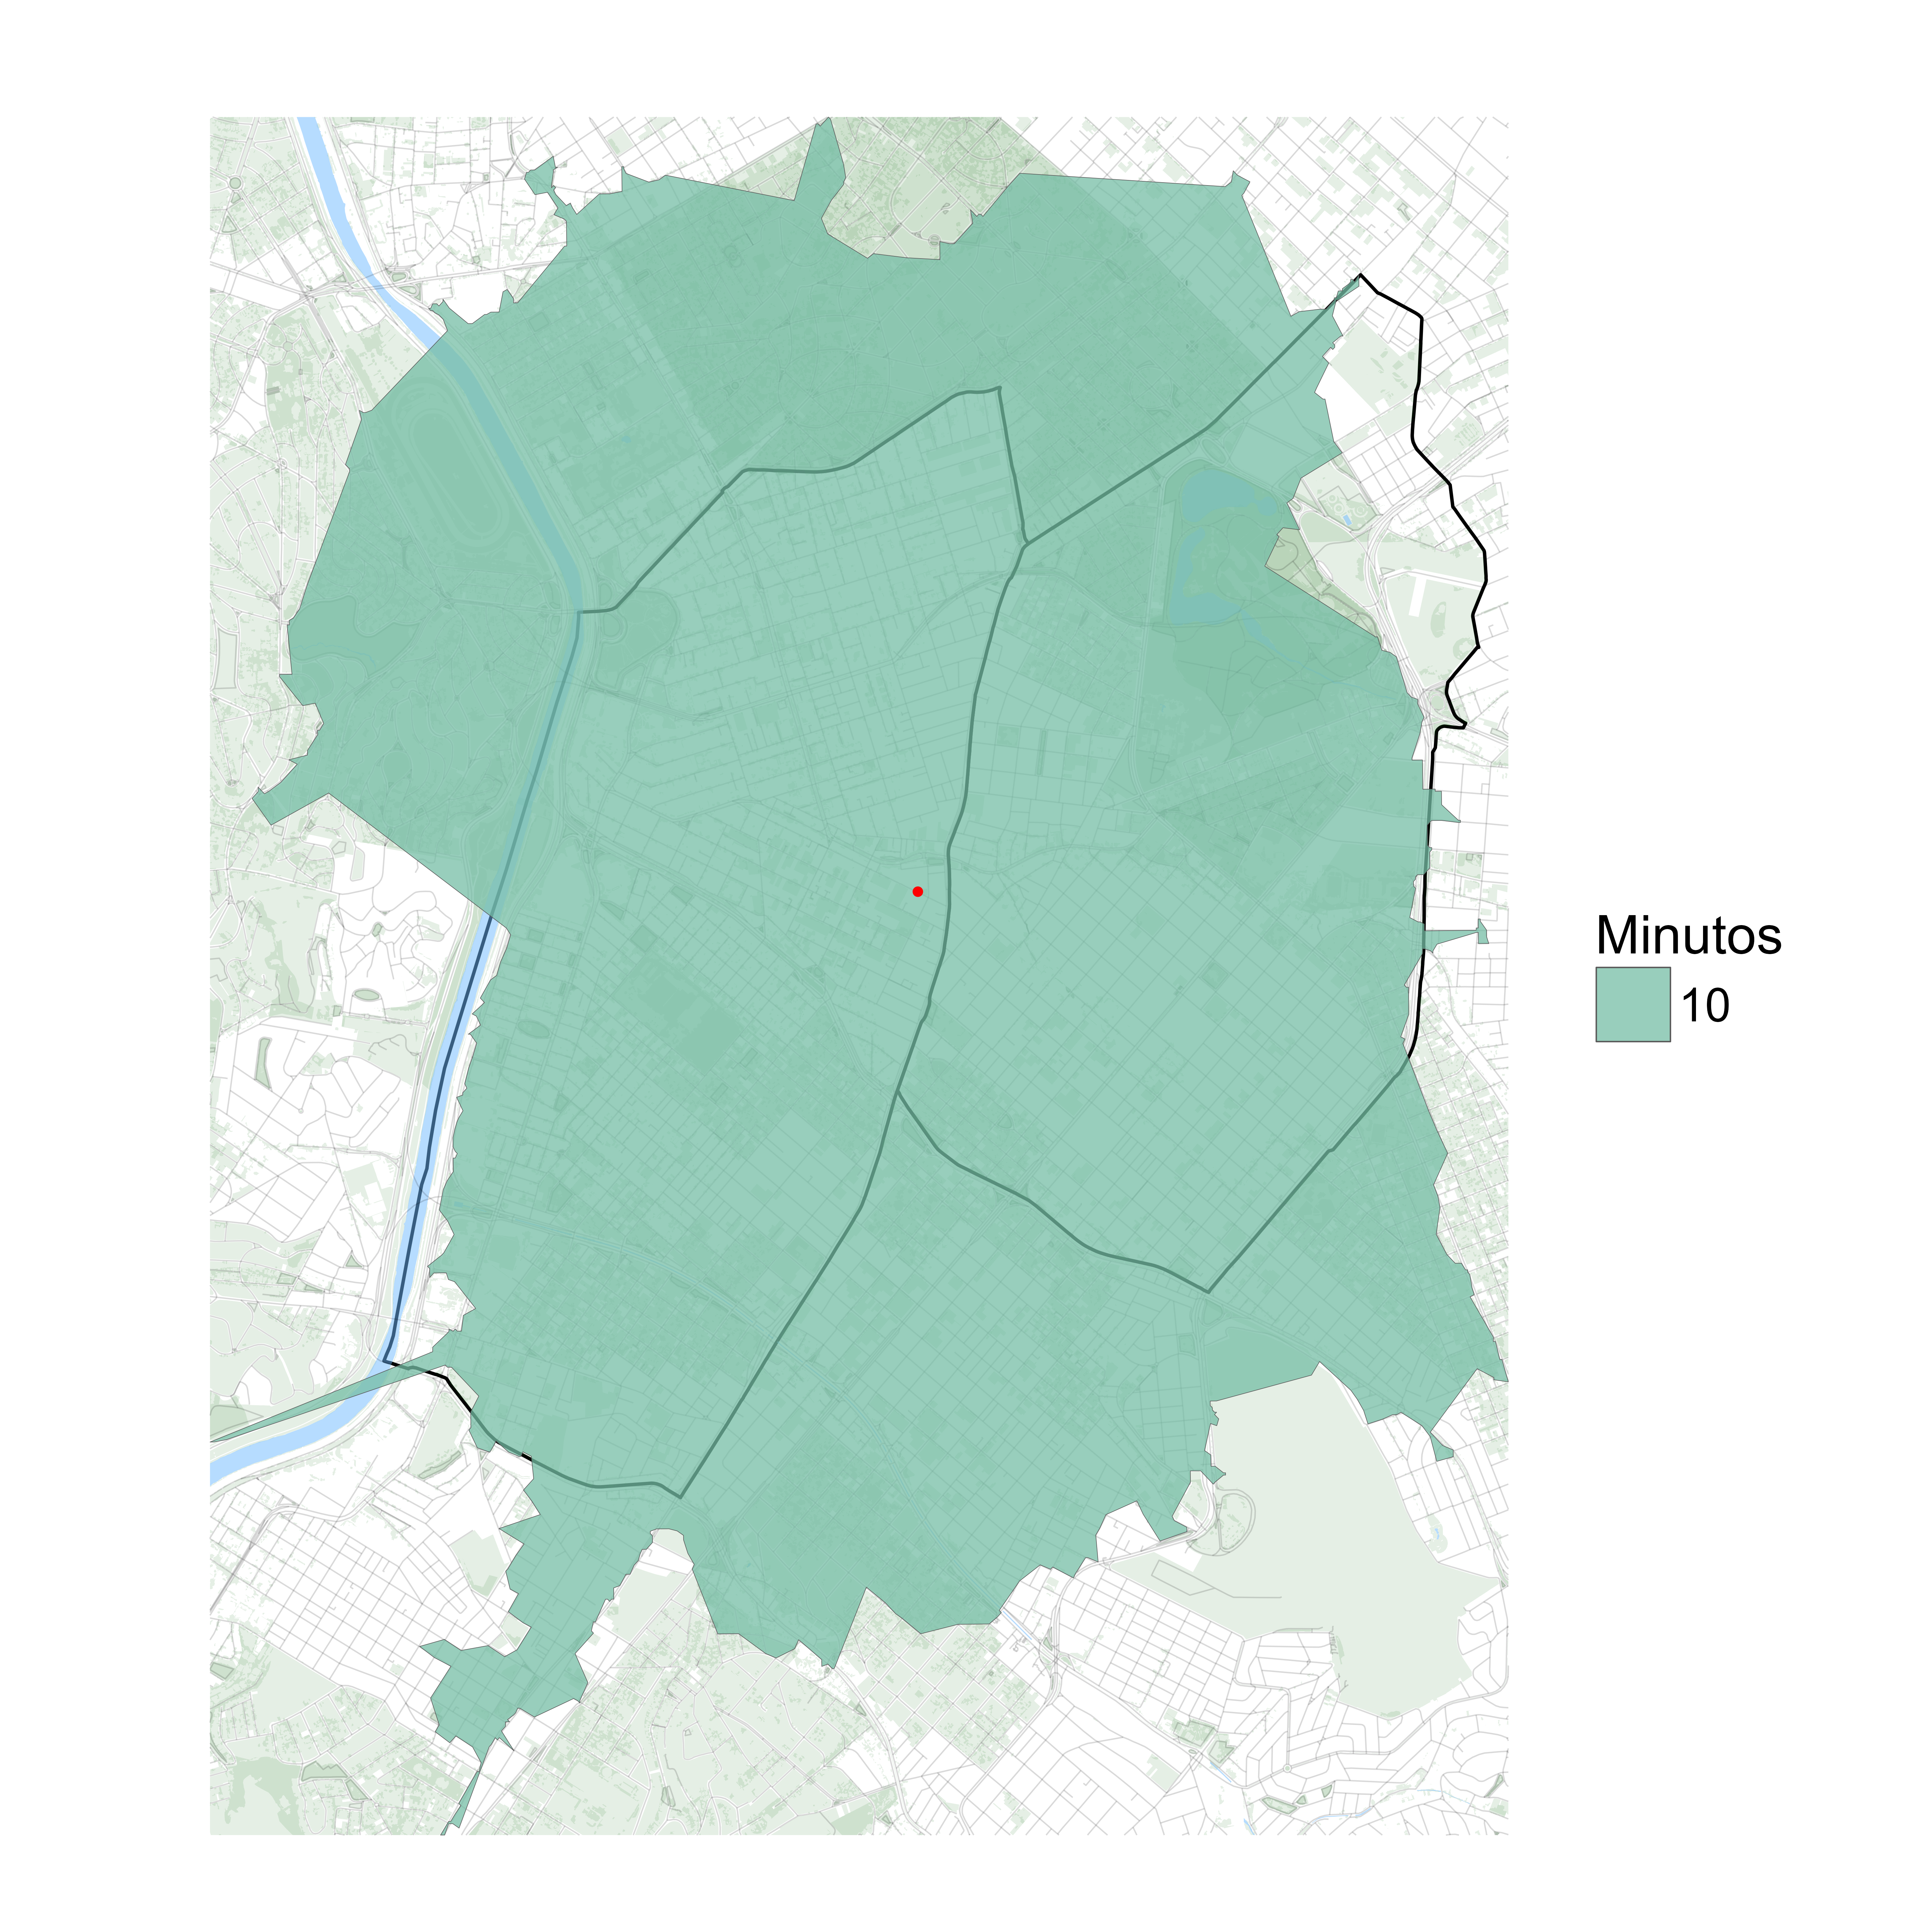
\includegraphics[width = 0.8\linewidth]{relatorios/uberabinha/figuras/car_S_uber_FINAL.png}
    \label{fig:iso_car_S}
\end{figure}

\begin{figure}[H]
    \centering
    \caption{Isócrona Bicicleta com intervenção na Rua Uberabinha}
    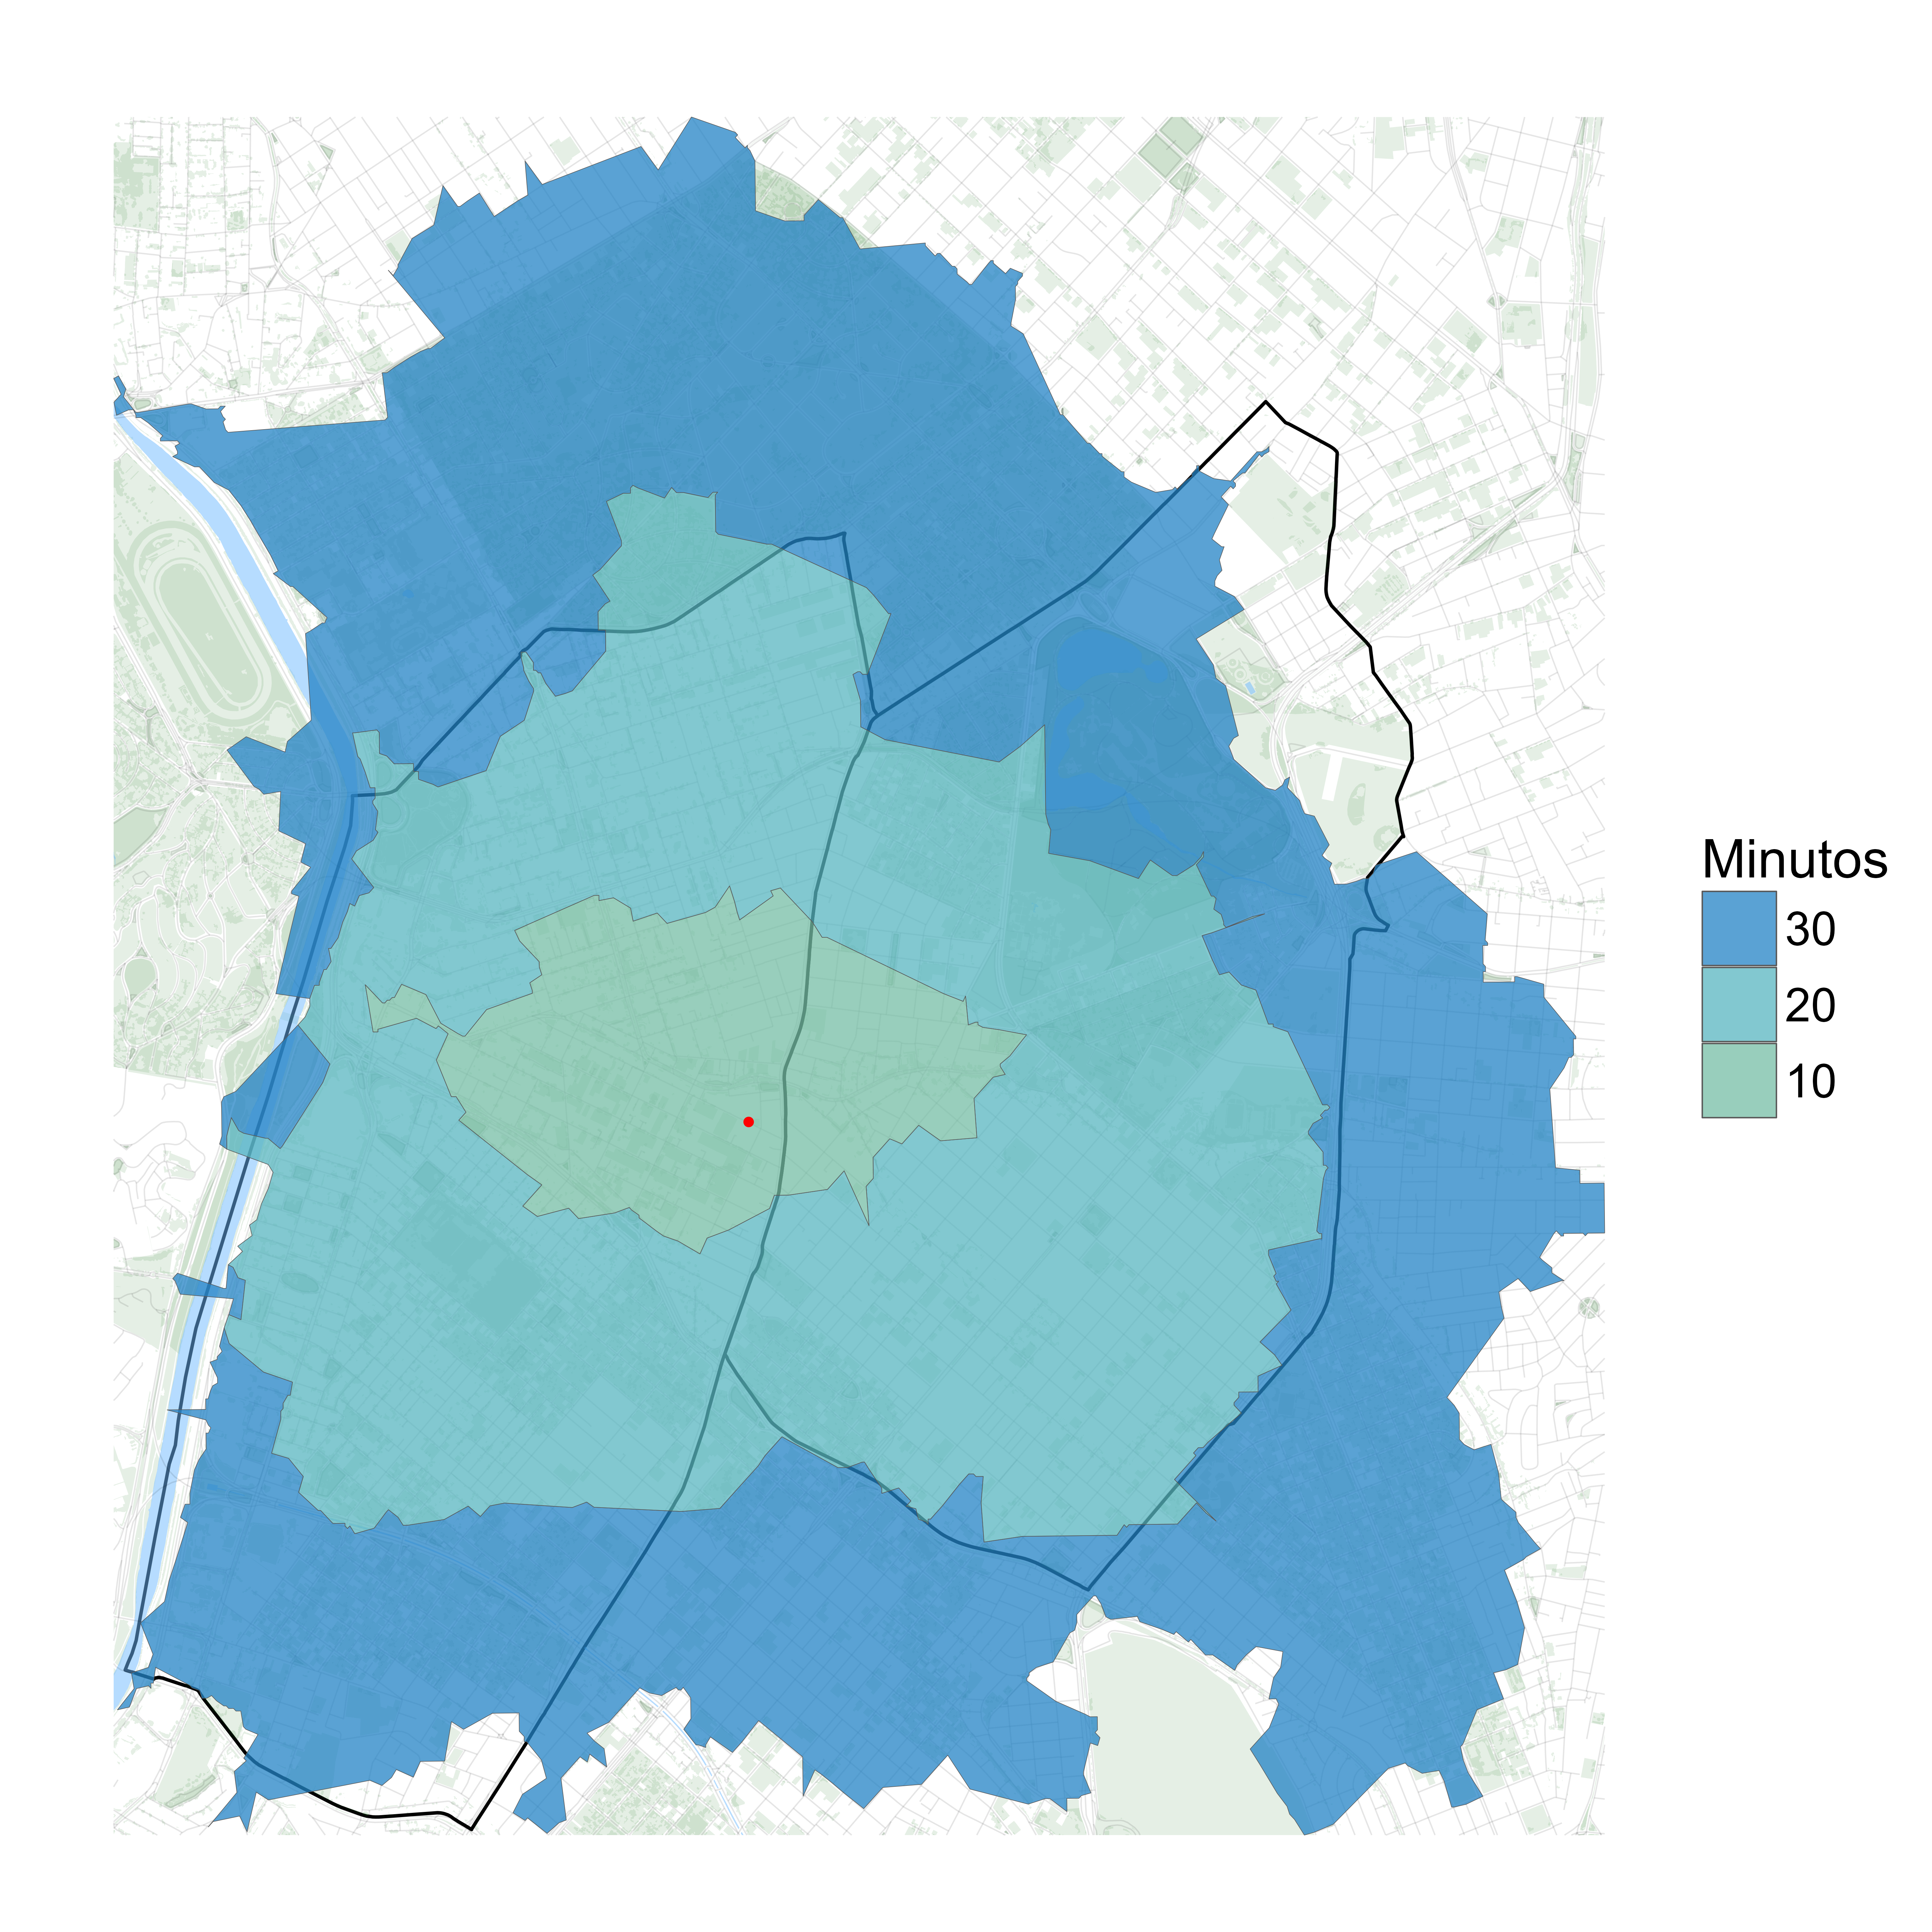
\includegraphics[width = 0.8\linewidth]{relatorios/uberabinha/figuras/bike_S_uber_FINAL.png}
    \label{fig:iso_bike_S}
\end{figure}

\begin{figure}[H]
    \centering
    \caption{Isócrona Pedestre sem intervenção na Rua Uberabinha}
    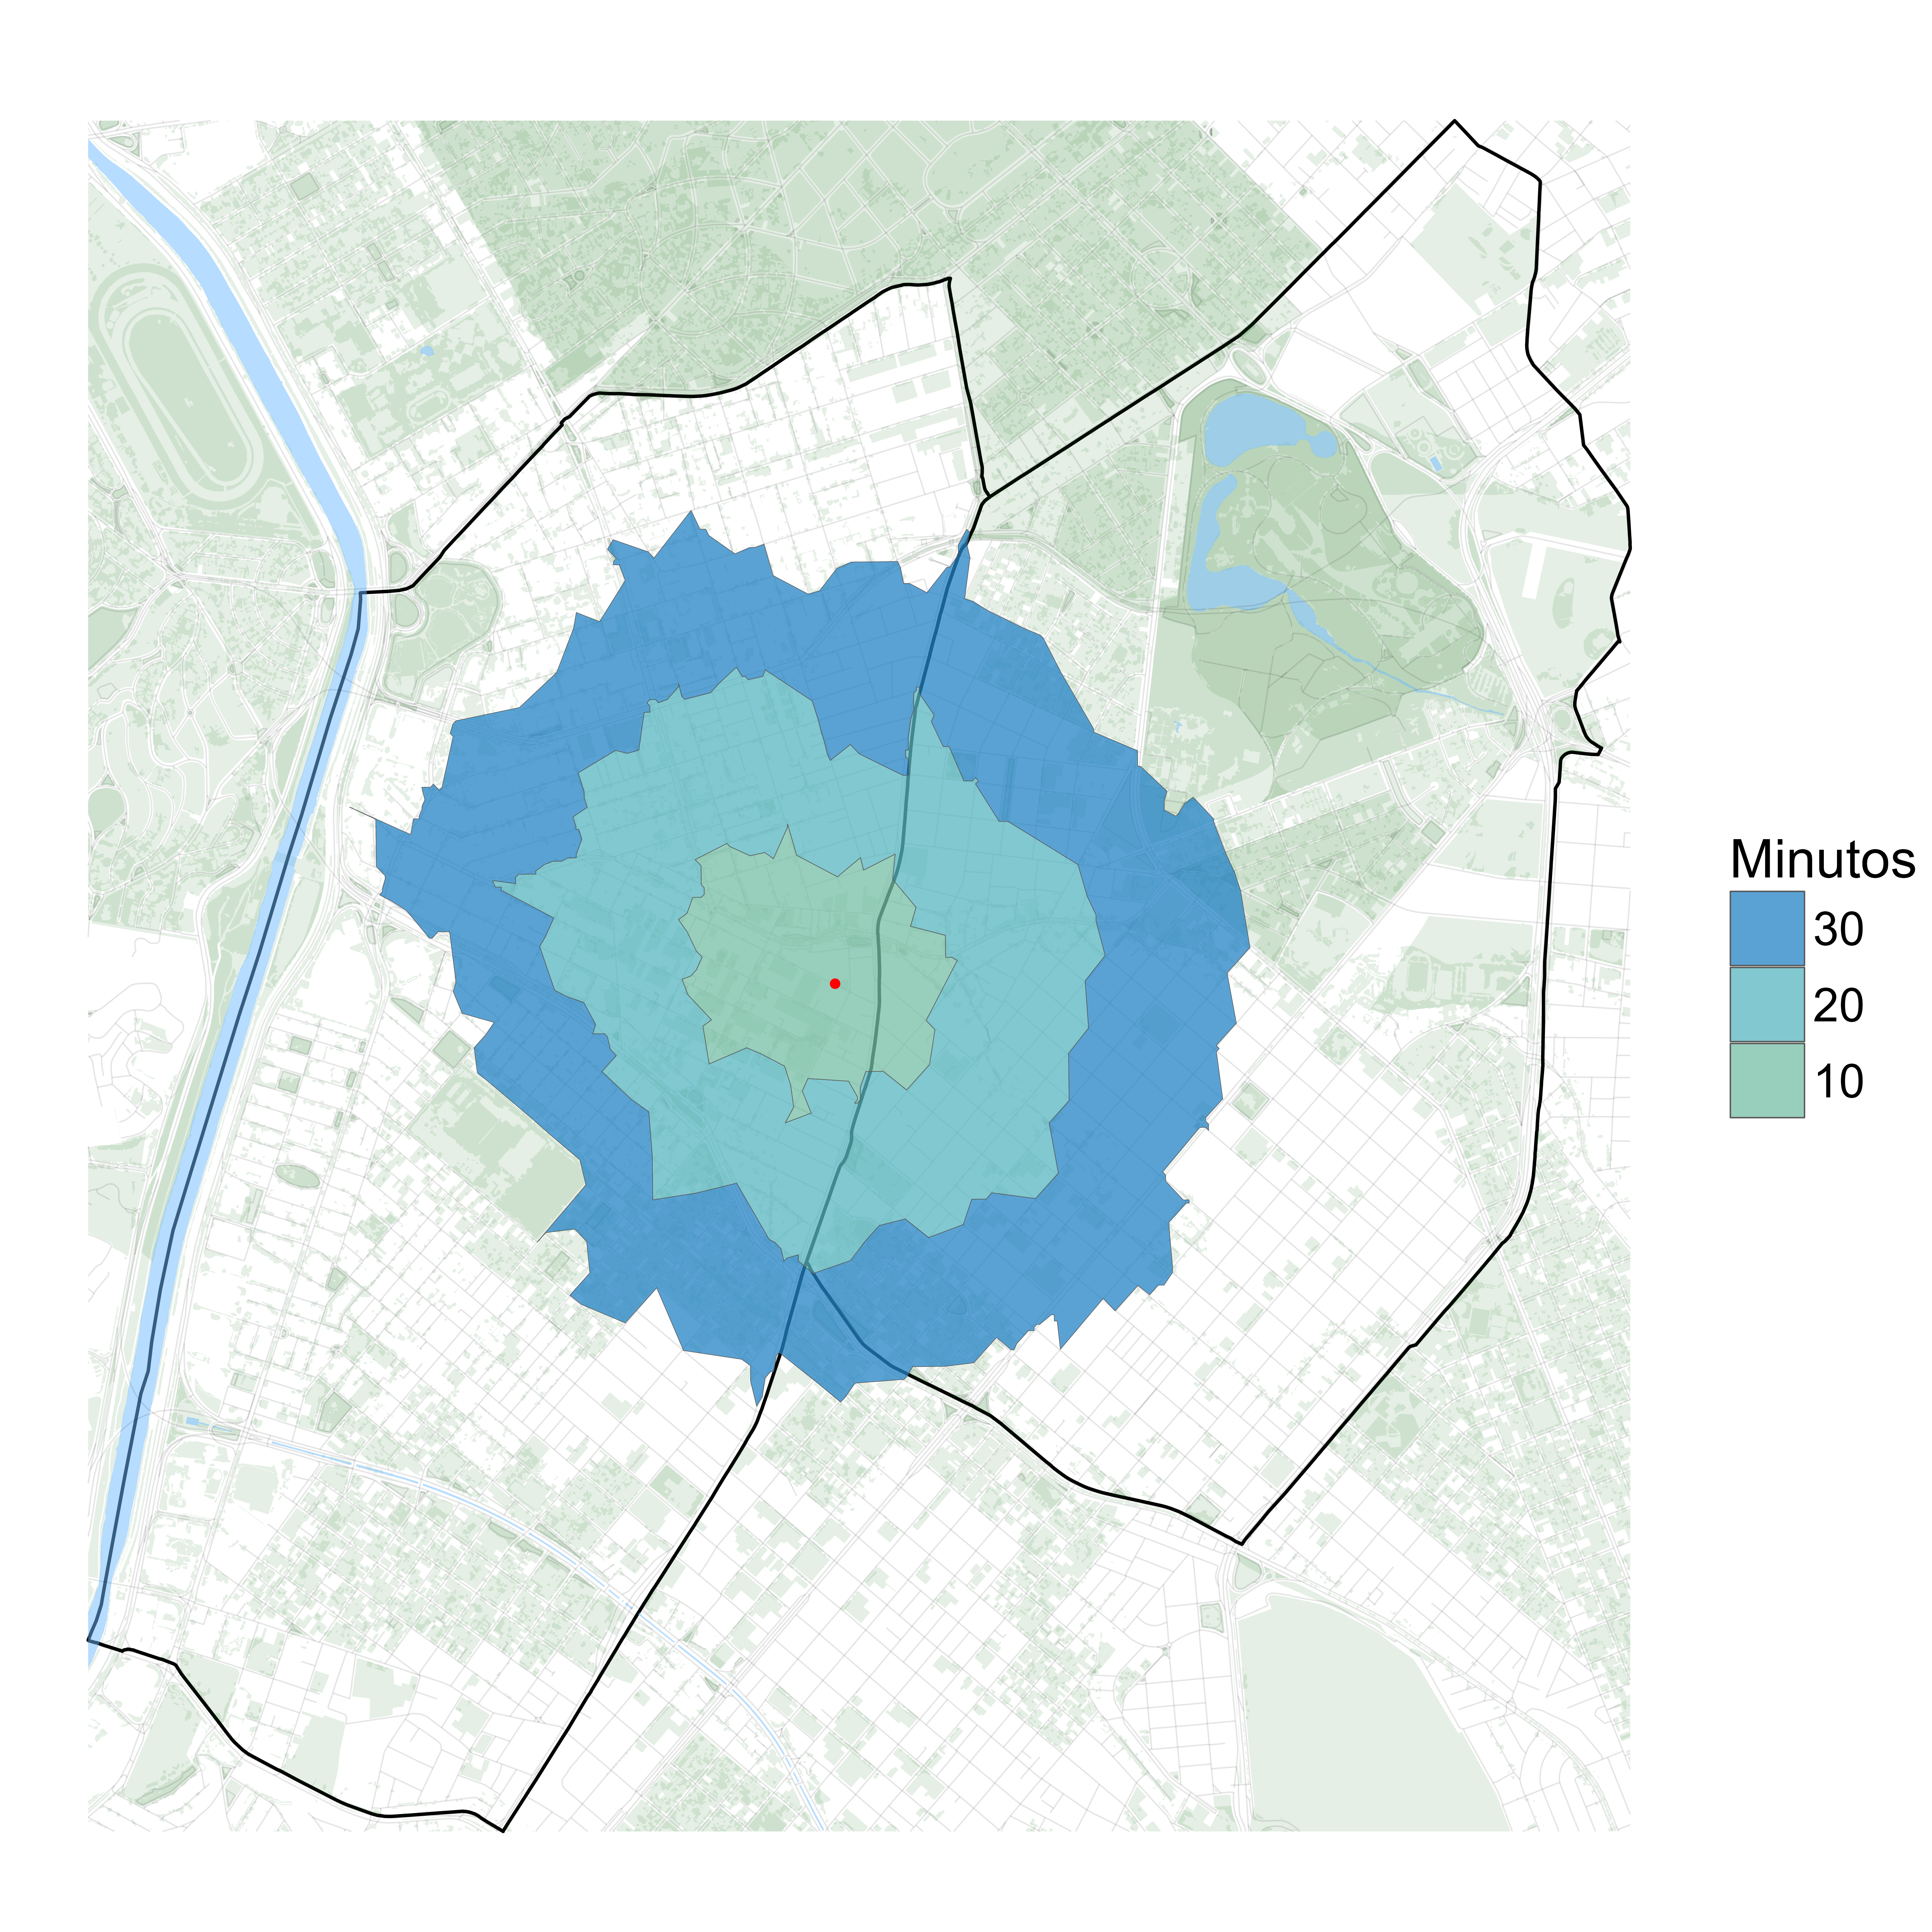
\includegraphics[width = 0.8\linewidth]{relatorios/uberabinha/figuras/walk_S_uber_FINAL.png}
    \label{fig:iso_pe_S}
\end{figure}

Sobre a análise descritiva das oportunidades ao redor do Insper, foram utilizados os resultados das rotas oferecidas pelo Maps, para conseguir notar a importância da Rua Uberabinha no deslocamento de cada modal ao redor da área analisada. Dessa forma, foram construídos mapas para cada modalidade de transporte, onde estes separam as oportunidades entre dependentes da Rua Uberabinha ou não, no melhor caminho fornecido pelo Google Maps. 

A partir das Figuras \ref{fig:oportunidades_carro}, \ref{fig:oportunidades_bike}, \ref{fig:oportunidades_pe}, pode-se notar a presença de regiões específicas que seriam mais afetadas pela mudança na Rua Uberabinha, com grande diferença entre quais oportunidades seriam afetadas dependendo da modalidade de transporte. Não só isso, como de forma visual, é evidente que os pedestres possuem menos oportunidades dependendo da Rua Uberabinha em seu melhor caminho.

\begin{figure}[H]
    \centering
    \caption{Mapa de oportunidades dependentes da Rua Uberabinha para Carro}
    \includegraphics[width = 0.8\linewidth]{relatorios/uberabinha/figuras/carro_FINAL.png}
    \label{fig:oportunidades_carro}
\end{figure}

\begin{figure}[H]
    \centering
    \caption{Mapa de oportunidades dependentes da Rua Uberabinha para Bicicleta}
    \includegraphics[width = 0.8\linewidth]{relatorios/uberabinha/figuras/bike_FINAL.png}
    \label{fig:oportunidades_bike}
\end{figure}

\begin{figure}[H]
    \centering
    \caption{Mapa de oportunidades dependentes da Rua Uberabinha para Pedestre}
    \includegraphics[width = 0.8\linewidth]{relatorios/uberabinha/figuras/pe_FINAL.png}
    \label{fig:oportunidades_pe}
\end{figure}

Partindo para a análise detalhada dos restaurantes em um raio de 1Km do Insper, estes apresentam boa repercussão de acordo com as avaliações do Google Maps. Alguns deles não possuíam notas, no entanto, dentre os detentores de avaliação, esses possuíam sua maior concentração entre o intervalo de 3,5 - 5. Assim sendo, é possível entender que os indivíduos que frequentam diariamente a região não possuem necessidade de grande deslocamentos para realizar uma refeição, pelo menos não pela qualidade do estabelecimentos.

\begin{figure}[H]
    \centering
    \caption{Mapa de restaurantes no raio de 1Km com avaliaçãos do Google Maps}
    \includegraphics[width = 0.8\linewidth]{relatorios/uberabinha/figuras/rating_FINAL.png}
    \label{fig:rating}
\end{figure}

\begin{figure}[H]
    \centering
    \caption{Acessibilidade pedestres para oportunidades selecionadas}
    \includegraphics[width = 0.8\linewidth]{relatorios/uberabinha/figuras/acessibilidade_pedestres.png}
    \label{fig:acessibilidade_pedestre}
\end{figure}

Com base no mapeamento de todas as oportunidades, foram selecionados quatro tipos de estabelecimentos - Café, Academia, Supermercado e Restaurante - para uma análise mais aprofundada sobre o acesso de pedestres aos tipos de oportunidade citados. O que foi observado em tal análise é que o acesso dos pedestres as oportunidades selecionadas é considerável, sem necessitar de um deslocamento de mais de 10 minutos, uma vez que neste ponto o indivíduo já teria alcançado: 51 restaurantes; 12 academias; 9 cafés e 6 supermercados.

\section{Conclusão}
Após análise da hipótese sobre como uma intervenção na Rua Uberabinha afetaria a acessibilidade das três modalidades de transporte: carro, pedestres e ciclistas, é possível concluir alguns aspectos.

Primeiramente, sobre a análise das isócronas antes e depois de uma alteração viária, sem considerar o trânsito na modelagem, é possível concluir que tal alteração não teria impacto significativo na área de alcance de nenhum dos transportes.

Além disso, a partir do mapeamento de todas as oportunidades em um raio de 3Km do Insper, e análise sobre quais oportunidades utilizam a Rua Uberabinha no seu melhor caminho - de acordo com o Google Maps - juntamente com o modelo teórico de Koenig, é possível concluir que: Caso fosse feita uma alteração viária, 30,78\% dos caminhos de pedestres e 61,19\% de ciclistas teriam a possibilidade de serem beneficiados, enquanto colocaria 69,10\% dos melhores caminhos para carros em risco de prejuízos.

Como citado anteriormente, uma limitação de tal estudo é a não implementação da análise do trânsito em nenhum dos resultados, justamente pela extensão da complexidade de tal elemento, o qual não era o foco da pesquisa.

A partir dos resultados encontrados e limitações do estudo, possíveis próximos passos para continuidade de tal análise seriam: simulação do fluxo viário aos arredores do Insper após a intervenção, contabilizando as mudanças de escolha dos indivíduos e o trânsito; simulação de alterações nos sentidos viários dos logradouros da região em busca do melhor arranjo caso a intervenção ocorresse e compreensão da importância das oportunidades beneficiadas e prejudicadas para cada tipo de transporte, buscando mensurar de forma mais completa quantos indivíduos estariam sendo beneficiados e prejudicados.

% \printbibliography[keyword=uberabinha]


\printbibliography[keyword = uberabinha]

\section{Apêndice}

\begin{figure}[h]
    \centering
    \caption{Mapeamento oportunidades no raio de 3Km}
    \includegraphics[width = 0.7\linewidth]{relatorios/uberabinha/figuras/oportunidades_FINAL.png}
\end{figure}

\begin{table}[h]
    \centering
    \caption{Mapeamento Oportunidades no raio de 3Km}

    \begin{tabular}{rlr}
        & Tipo & Contagem \\ 
        \hline

        1 & store & 3755 \\ 
          2 & restaurant & 1817 \\ 
          3 & beauty\_salon & 1035 \\ 
          4 & school & 692 \\ 
          5 & car\_repair & 619 \\ 
          6 & bar & 560 \\ 
          7 & gym & 473 \\ 
          8 & hospital & 425 \\ 
          9 & café & 340 \\ 
          10 & bank & 282 \\ 
          11 & car\_dealer & 238 \\ 
          12 & market & 142 \\ 
          13 & university & 120 \\ 
          14 & supermarket &  94 \\ 
          15 & gas\_station &  70 \\ 
          16 & shopping\_mall &  56 \\ 
          17 & police &  16 \\ 
          18 & fire\_station &   6 \\ 
        
           \hline
    \end{tabular}
    \label{tab_oportunidades}
\end{table}



    

\begin{figure}[h]
    \centering
    \caption{Acessibilidade das modalidades de transporte}
    \includegraphics[width = 0.7\linewidth]{relatorios/uberabinha/figuras/acessibilidade_por_modal.png}
\end{figure}

\begin{figure}[h]
    \centering
    \caption{Dados da coleta manual no local de estudo}
    \includegraphics[width = 0.7\linewidth]{relatorios/uberabinha/figuras/Teste.png}
\end{figure}


